\chapter{M�todos demogr�ficos para poblaciones peque�as}


\section{Selecci�n de variables}

Aunque es posible usar los m�todos demogr�ficos para realizar proyecciones fuera del intervalo de medici�n, su uso m�s frecuente es realizar interpolaci�n de poblaciones peque�as en periodos no censales. Uno de los inconvenientes mencionados es la dificultad de realizar extrapolaci�n, puesto que para los periodos post-censales, los indicadores no est�n necesariamente disponibles. Una posible soluci�n es realizar la estimaci�n usando periodos rezagados. \cite{Swanson2012}. 

Para realizar la proyecci�n a tres a�os, como en el cap�tulo anterior, se utilizan variables que tengan una proyecci�n oficial, por lo menos anual para los siguientes tres a�os. La metodolog�a de proyecci�n de Blumstein sugiere que bajo un sistema normativo estable, la proporci�n de la poblaci�n carcelaria por rango etario resulta fundamental en la proyecci�n de poblaciones carcelarias \cite{Blumstein1980a}. Dado que el DANE genera poblaciones de poblaci�n desagregadas por rango etario, usaremos estas en el m�todo de ratio-correlaci�n.

% Es posible copiar la tabla completa. 

\section{Poblaci�n colombiana 1991-2020}

\begin{figure}[H]
	\centering
	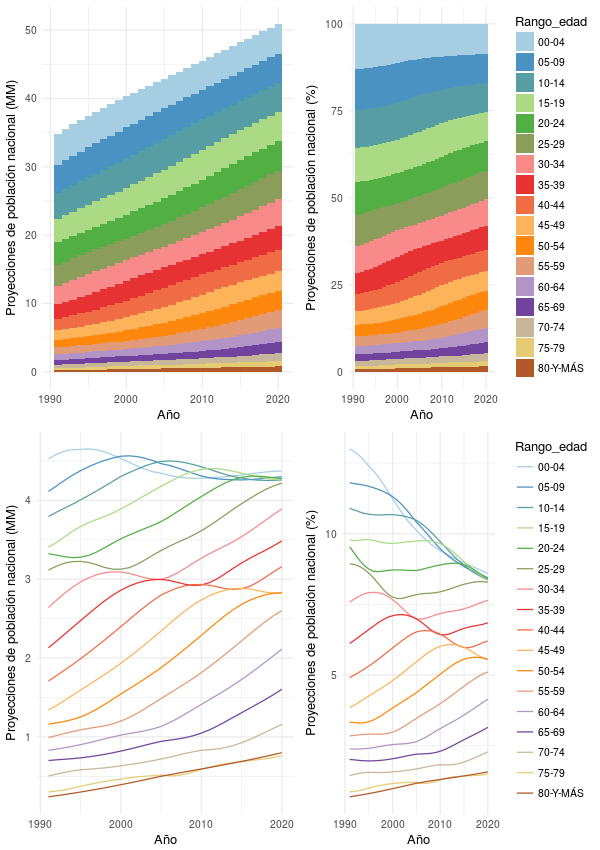
\includegraphics[width=0.7\linewidth]{POB_NAL_EDAD.png}
	\caption[Proyecci�n de la poblaci�n nacional por rango de edad]{Proyecci�n de la poblaci�n nacional por rango de edad}{Fuente: DANE\\} {Elaboraci�n propia}
	\label{fig:pob_nal_dane_edad}
\end{figure}

